\documentclass[12pt,a4paper]{article}

% ── Packages ──────────────────────────────────────────────────────────────────
\usepackage[top=2.5cm, bottom=2.5cm, left=2.5cm, right=2.5cm]{geometry}
\usepackage{tikz}
\usetikzlibrary{shapes.geometric, arrows.meta, positioning, fit, backgrounds, calc}
\usepackage{xcolor}
\usepackage{booktabs}
\usepackage{tabularx}
\usepackage{array}
\usepackage{longtable}
\usepackage{hyperref}
\usepackage{enumitem}
\usepackage{titlesec}
\usepackage{fancyhdr}
\usepackage{parskip}
\usepackage[T1]{fontenc}
\usepackage{amssymb}
\usepackage{listings}
\usepackage{caption}
\usepackage{float}
\usepackage{graphicx}
\usepackage{subcaption}
\usepackage{amsmath}

% ── Colours ───────────────────────────────────────────────────────────────────
\definecolor{clientblue}{RGB}{210,228,255}
\definecolor{gatewaygreen}{RGB}{210,240,220}
\definecolor{svcyellow}{RGB}{255,249,210}
\definecolor{dbgray}{RGB}{225,225,225}
\definecolor{mqorange}{RGB}{255,232,210}
\definecolor{redisred}{RGB}{255,218,218}
\definecolor{bordercolor}{RGB}{80,80,80}
\definecolor{accentblack}{RGB}{0,0,0}
\definecolor{lightgray}{RGB}{245,245,245}
\definecolor{tablegray}{RGB}{240,240,240}
\definecolor{gridgreen}{RGB}{200,240,200}
\definecolor{routepurple}{RGB}{220,200,255}

% ── Section styling ──────────────────────────────────────────────────────────
\titleformat{\section}{\large\bfseries\color{black}}{{\thesection}}{1em}{}[\titlerule]
\titleformat{\subsection}{\normalsize\bfseries\color{black}}{{\thesubsection}}{1em}{}
\titleformat{\subsubsection}{\normalsize\itshape\color{black}}{{\thesubsubsection}}{1em}{}

% ── Header / Footer ──────────────────────────────────────────────────────────
\pagestyle{fancy}
\fancyhf{}
\lhead{\small\textbf{Journey Booking System --- Final Report}}
\rhead{\small CS7NS6 --- Exercise 2 --- Group J}
\cfoot{\thepage}
\renewcommand{\headrulewidth}{0.4pt}

% ── Hyperref ─────────────────────────────────────────────────────────────────
\hypersetup{
  colorlinks=true,
  linkcolor=black,
  urlcolor=black,
  citecolor=black,
  pdftitle={Journey Booking System --- Final Technical Report},
}

% ── Table helpers ─────────────────────────────────────────────────────────────
\newcolumntype{L}[1]{>{\raggedright\arraybackslash}p{#1}}
\newcolumntype{C}[1]{>{\centering\arraybackslash}p{#1}}

% ── Code listing style ────────────────────────────────────────────────────────
\lstset{
  basicstyle=\ttfamily\small,
  breaklines=true,
  frame=single,
  framerule=0.4pt,
  rulecolor=\color{black},
  backgroundcolor=\color{lightgray},
  keywordstyle=\bfseries,
}

% ── TikZ styles ───────────────────────────────────────────────────────────────
\tikzset{
  base/.style={draw=bordercolor, line width=0.8pt, align=center,
               font=\small, minimum height=1cm},
  client/.style   = {base, rounded corners=6pt, fill=clientblue,  minimum width=3.2cm},
  gateway/.style  = {base, rounded corners=6pt, fill=gatewaygreen, minimum width=6cm, minimum height=1.4cm},
  service/.style  = {base, rounded corners=4pt, fill=svcyellow,   minimum width=2.6cm},
  database/.style = {base, cylinder, shape border rotate=90, aspect=0.3,
                     fill=dbgray, minimum width=2cm, minimum height=1cm},
  broker/.style   = {base, rounded corners=4pt, fill=mqorange,    minimum width=2.8cm},
  cache/.style    = {base, cylinder, shape border rotate=90, aspect=0.3,
                     fill=redisred, minimum width=2cm, minimum height=1cm},
  region/.style   = {base, rounded corners=4pt, fill=gridgreen,   minimum width=3cm},
  arr/.style      = {-{Stealth[length=5pt]}, line width=0.8pt, color=bordercolor},
  darr/.style     = {-{Stealth[length=5pt]}, line width=0.7pt, dashed, color=bordercolor},
}

% ─────────────────────────────────────────────────────────────────────────────
\begin{document}

% ── Title Page ────────────────────────────────────────────────────────────────
\begin{titlepage}
  \centering
  \vspace*{2cm}
  {\LARGE\bfseries Journey Booking System\par}
  \vspace{0.4cm}
  {\Large Final Technical Architecture Report\par}
  \vspace{1.5cm}
  \rule{0.6\textwidth}{0.4pt}\par
  \vspace{0.8cm}
  {\large\textbf{Module:} CS7NS6 Distributed Systems --- Exercise 2\par}
  \vspace{0.3cm}
  {\large\textbf{Group:} J\par}
  \vspace{0.3cm}
  {\large\textbf{Date:} April 2026\par}
  \vspace{2cm}

  \begin{tabular}{m{4.5cm} m{6cm}}
    \toprule
    \textbf{Name} & \textbf{Service Responsibility} \\
    \midrule
    Parth Deshmukh         & User Service \\\addlinespace[0.4cm]
    Tanmay Ghosh           & Journey Service \\\addlinespace[0.4cm]
    Sneha Meto             & Conflict Detection Service \\\addlinespace[0.4cm]
    Aditya Kumar Singh     & Notification Service \\\addlinespace[0.4cm]
    Saurabh Deshmukh       & Enforcement Service \\\addlinespace[0.4cm]
    Sai Eeshwar Divaakar   & Analytics \& Monitoring Service \\\addlinespace[0.4cm]
    \bottomrule
  \end{tabular}
\end{titlepage}

% ── Table of Contents ─────────────────────────────────────────────────────────
\tableofcontents
\newpage

% ─────────────────────────────────────────────────────────────────────────────
\section{Introduction}

This report describes the final implementation of a globally-accessible journey pre-booking system for road-vehicle drivers. The system allows drivers to reserve road access before they travel: no driver may start a journey without a confirmed booking. Roadside enforcement agents verify active bookings in real time.

The system is structured as six independently deployable microservices. This final report explicitly addresses four areas raised in the interim review:
\begin{enumerate}[leftmargin=*]
  \item \textbf{Geographic distribution and data partitioning} --- how the system supports multi-region deployment and how road-capacity data is spatially partitioned.
  \item \textbf{Multi-national journey consistency} --- how journeys that cross regional or national boundaries are handled atomically.
  \item \textbf{Reliability and consistency} --- the explicit use of ACID transactions, pessimistic locking, streaming replication, and the saga/outbox pattern.
  \item \textbf{Road map management and routing} --- where route computation happens, how the road network is queried, and how route geometry flows through the system.
\end{enumerate}

% ─────────────────────────────────────────────────────────────────────────────
\section{System Architecture}

\subsection{High-Level Overview}

\begin{figure}[H]
  \centering
  % Replace with your actual architecture diagram
  \includegraphics[width=\textwidth]{images/booking-architecture.png}
  \caption{Full system architecture. Each service owns its own database and
           communicates asynchronously via RabbitMQ after the initial synchronous saga call.}
  \label{fig:architecture}
\end{figure}

All client traffic enters through an \textbf{HAProxy $\to$ Nginx} gateway pair. Nginx enforces per-zone rate limiting and routes requests to the appropriate upstream service. Two Nginx instances sit behind HAProxy for gateway-layer redundancy.

\subsection{Service Decomposition}

\begin{table}[H]
\centering
\small
\begin{tabularx}{\textwidth}{C{0.4cm} L{3cm} X L{2.8cm} C{1.4cm}}
  \toprule
  \textbf{\#} & \textbf{Service} & \textbf{Responsibility} & \textbf{Database} & \textbf{Language} \\
  \midrule
  1 & User Service        & Registration, JWT authentication, driver profiles, vehicle registry
    & PostgreSQL + replica & Python \\
  \addlinespace[0.15cm]
  2 & Journey Service     & Journey CRUD, booking saga, transactional outbox, OSRM route computation, idempotency, points ledger
    & PostgreSQL + replica & Python \\
  \addlinespace[0.15cm]
  3 & Conflict Detection  & Time-overlap, vehicle-overlap, geographic road-capacity checking per grid cell
    & PostgreSQL           & Go \\
  \addlinespace[0.15cm]
  4 & Notification Service& Event consumption, WebSocket push, notification history
    & Redis                & Go \\
  \addlinespace[0.15cm]
  5 & Enforcement Service & Active booking verification by plate or licence; Redis-first with HTTP fallback
    & Redis cache          & Python \\
  \addlinespace[0.15cm]
  6 & Analytics Service   & Event logging, hourly rollup aggregation, HMAC audit trail, system health aggregation
    & PostgreSQL + replica + Redis & Go \\
  \bottomrule
\end{tabularx}
\caption{Service decomposition. Each service owns its own database (database-per-service pattern).}
\end{table}

\subsection{Communication Patterns}

The system uses two distinct communication styles:

\begin{itemize}[leftmargin=*]
  \item \textbf{Synchronous REST} --- Journey Service calls Conflict Detection Service during booking. This is a deliberate saga step that must complete before a decision can be made.
  \item \textbf{Asynchronous messaging (RabbitMQ)} --- After a journey is confirmed, rejected, or cancelled, the Journey Service writes an event to a transactional outbox. A background publisher drains this to a RabbitMQ topic exchange. Downstream consumers (Notification, Enforcement, Analytics, Conflict) process events independently.
\end{itemize}

\textbf{Booking request path:}

\begin{lstlisting}
Client -> Nginx -> Journey Service
  -> Conflict Detection Service (sync REST, saga step)
  <- approved / rejected
  -> DB: write journey + outbox event (same ACID transaction)
  -> background drain: outbox -> RabbitMQ topic exchange
  ~> Notification Service (WebSocket push)
  ~> Enforcement Service (cache update)
  ~> Analytics Service (event log + Redis counter)
  ~> Conflict Detection (slot reservation confirmed)
\end{lstlisting}

% ─────────────────────────────────────────────────────────────────────────────
\section{Geographic Distribution and Data Partitioning}

\subsection{Road Segment Grid Partitioning}

The Conflict Detection Service is the component responsible for geographic data. It does not treat road capacity as a single global resource. Instead, it applies a \textbf{geographic grid model}: the road network is divided into cells defined by latitude/longitude bounding boxes of approximately $0.01°$ per side (${\approx}1\,\text{km}^2$ at European latitudes). Each grid cell tracks:

\begin{itemize}[leftmargin=*]
  \item Current vehicle count (how many active journeys pass through this cell)
  \item Maximum road capacity (configurable per cell, defaulting to a system-wide constant)
\end{itemize}

When a booking request arrives, the Journey Service provides the full route geometry (a GeoJSON LineString returned by OSRM). The Conflict Detection Service walks the route coordinates, maps each coordinate to its grid cell using integer floor division of latitude and longitude, and checks capacity for every cell the route passes through. A booking is confirmed only if \emph{all} cells along the route have remaining capacity.

This partitioning is the foundation for geographic scalability:

\begin{itemize}[leftmargin=*]
  \item Capacity checks for routes in Ireland are independent of checks for routes in France.
  \item Different instances of the Conflict Detection Service could own different geographic ranges (e.g.\ shard by $\lfloor \text{lat} \rfloor$) without any change to the booking logic.
  \item The grid cell key space is deterministic and shardable by consistent hashing.
\end{itemize}

\subsection{Multi-Region Deployment Model}

The system is designed to run split across machines. The recommended deployment separates infrastructure (RabbitMQ, Redis, PostgreSQL) onto one machine and application services onto another, connected over a network:

\begin{figure}[H]
\centering
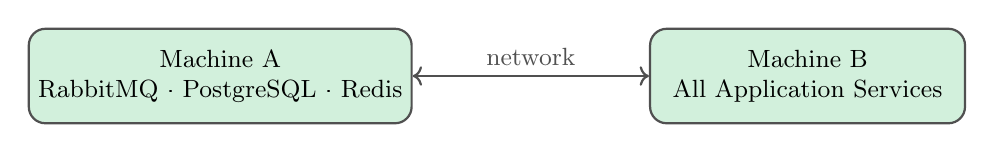
\begin{tikzpicture}[node distance=0.8cm and 1.5cm]
  \node[gateway, minimum width=4cm, minimum height=1.2cm] (machA) {Machine A\\{\small RabbitMQ · PostgreSQL · Redis}};
  \node[gateway, minimum width=4cm, minimum height=1.2cm, right=3cm of machA] (machB) {Machine B\\{\small All Application Services}};
  \draw[arr, <->] (machA) -- node[above, font=\small]{network} (machB);
\end{tikzpicture}
\caption{Two-machine deployment for demonstration. Killing Machine A mid-demo exercises the circuit breaker and transactional outbox.}
\end{figure}

In a full multi-region deployment (e.g.\ Ireland / UK / France), each region would run its own set of services with its own PostgreSQL primary. Cross-region bookings would be routed to the authoritative Conflict Detection instance for each geographic shard, with the Journey Service saga coordinating the distributed approval.

\subsection{Multi-National Journey Consistency}

A journey from Dublin to London crosses the Irish Sea and enters UK road network. With the OSRM route geometry available at booking time, the Conflict Detection Service checks grid cells in both Ireland (\texttt{IE}) and the United Kingdom (\texttt{GB}):

\begin{enumerate}[leftmargin=*]
  \item The Journey Service calls Conflict Detection with the full GeoJSON route.
  \item Conflict Detection iterates all route coordinates, grouping them by grid cell.
  \item Cells in both countries are checked atomically within a single PostgreSQL transaction using \texttt{SELECT FOR UPDATE} on the capacity rows.
  \item If any cell in any country is at capacity, the \emph{entire} booking is rejected. No partial approval is possible.
  \item On approval, all cell counts are incremented in the same transaction.
\end{enumerate}

This gives \textbf{all-or-nothing atomicity} across geographic boundaries. The trade-off is that the Conflict Detection Service must have visibility of all cells along the route, which in a sharded deployment would require a two-phase commit or saga compensation within the Conflict Service layer.

\subsection{Partition Detection and Staleness Headers}

The Journey Service runs a background \texttt{PartitionManager} that periodically probes its dependencies (PostgreSQL primary, RabbitMQ). If a probe fails, the service sets an internal \texttt{PARTITIONED} flag and begins attaching an \texttt{X-Partition-Detected: true} header to responses. The Enforcement Service does the same when it cannot reach Redis or the Journey Service. This allows clients and monitoring tools to observe partition events without requiring a separate control plane.

% ─────────────────────────────────────────────────────────────────────────────
\section{Road Network Routing}

\subsection{Where Routing Happens}

Routing is computed \textbf{server-side} in the Journey Service at booking time. We integrate with OSRM (Open Source Routing Machine), which uses OpenStreetMap road network data. The routing call is:

\begin{lstlisting}
GET https://router.project-osrm.org/route/v1/driving/
    {origin_lng},{origin_lat};{dest_lng},{dest_lat}
    ?overview=full&geometries=geojson
\end{lstlisting}

This returns a GeoJSON \texttt{LineString} with the complete road-network path between the two points. For a Dublin--Cork route, this yields approximately 3,500 coordinate points tracing the M7/M8 motorway.

\subsection{Route Storage and Propagation}

The route geometry is stored persistently with the journey record:

\begin{enumerate}[leftmargin=*]
  \item OSRM is called after the saga approves the booking.
  \item The GeoJSON geometry string is written to the \texttt{route\_geometry} column of the \texttt{journeys} table in the same commit as the status update to \texttt{CONFIRMED}.
  \item The geometry is included in the \texttt{JourneyResponse} schema and returned to the client in the \texttt{POST /api/journeys/} response.
  \item The outbox event payload carries \texttt{route\_geometry}, so it propagates to all downstream consumers via RabbitMQ.
  \item The Notification Service includes it in the WebSocket metadata, so the live map updates in real time on the correct road path without any additional client-side API call.
\end{enumerate}

\textbf{Resilience:} The OSRM call is best-effort with an 8-second timeout. If it fails (e.g.\ OSRM is unreachable), the booking proceeds with \texttt{route\_geometry = null}. The client frontend falls back to a live OSRM fetch on render, and if that also fails, it draws a straight line. The booking is never blocked by routing unavailability.

\subsection{Conflict Detection Uses Route Geometry}

Before this change, the Conflict Detection Service approximated route coverage from just the origin and destination coordinates. With the stored GeoJSON geometry, it can walk the \emph{actual road path} and check every grid cell the vehicle will physically pass through, eliminating false positives and false negatives caused by straight-line approximation.

% ─────────────────────────────────────────────────────────────────────────────
\section{Reliability, Consistency, and Transactions}

\subsection{ACID Transactions}

The system uses explicit database transactions at every write boundary:

\begin{table}[H]
\centering
\small
\begin{tabularx}{\textwidth}{L{3.5cm} X}
  \toprule
  \textbf{Operation} & \textbf{Transaction Scope} \\
  \midrule
  Journey creation    & Journey row + outbox event written atomically in one PostgreSQL transaction. If either write fails, neither is committed --- the outbox event is never lost relative to the journey state. \\
  \addlinespace[0.15cm]
  Journey cancellation& Status update to \texttt{CANCELLED} + outbox event in one transaction. \\
  \addlinespace[0.15cm]
  Points deduction    & \texttt{SELECT FOR UPDATE} on \texttt{driver\_points} row prevents concurrent requests from double-spending the same balance. \\
  \addlinespace[0.15cm]
  Conflict capacity check & \texttt{SELECT FOR UPDATE} on grid cell rows ensures that two concurrent bookings on the same segment cannot both pass the capacity check. \\
  \addlinespace[0.15cm]
  Hourly stats rollup & Idempotent \texttt{INSERT ... ON CONFLICT DO UPDATE} ensures rollup job is safe to re-run. \\
  \bottomrule
\end{tabularx}
\caption{Explicit transaction boundaries across the system.}
\end{table}

\subsection{Transactional Outbox Pattern}

The Journey Service uses the \textbf{transactional outbox pattern} to guarantee at-least-once event delivery to RabbitMQ:

\begin{enumerate}[leftmargin=*]
  \item An \texttt{OutboxEvent} row is written in the \emph{same database transaction} as the journey status update. The outbox event cannot exist without the corresponding journey state, and vice versa.
  \item A background thread polls the \texttt{outbox\_events} table for \texttt{published = false} rows and publishes them to RabbitMQ.
  \item On successful publish, the row is marked \texttt{published = true} in a separate commit.
  \item If the process crashes between publish and the DB commit, the event will be re-published on restart (at-least-once).
  \item If RabbitMQ is down, events accumulate in the outbox table and are drained automatically when the broker recovers.
\end{enumerate}

This is demonstrated in the demo by stopping RabbitMQ mid-booking: the booking succeeds, the event is buffered in the outbox, and all downstream services receive it when the broker restarts.

\subsection{Saga Pattern for Distributed Booking}

The booking saga is orchestrated by the Journey Service:

\begin{enumerate}[leftmargin=*]
  \item Journey created with status \texttt{PENDING}.
  \item Journey Service calls Conflict Detection Service synchronously (HTTP REST).
  \item Conflict Detection checks time overlap, vehicle overlap, and geographic road capacity.
  \item On approval: Journey Service updates status to \texttt{CONFIRMED} + writes outbox event.
  \item On rejection or timeout: Journey Service updates status to \texttt{REJECTED} + writes outbox event. No compensating transaction is needed because no resource was reserved.
\end{enumerate}

The circuit breaker (configured with 3 failures, 60-second open window) wraps the Conflict Detection call. When the circuit is open, booking requests fail fast with HTTP 503 rather than accumulating waiting threads.

\subsection{Database Replication}

Each PostgreSQL database runs with a \textbf{primary + streaming replica} pair configured in Docker Compose. Streaming replication transmits WAL segments from the primary to the replica in near real-time (typically $<5\,\text{ms}$ lag on a local network):

\begin{itemize}[leftmargin=*]
  \item \textbf{Writes} always go to the primary via \texttt{DATABASE\_URL}.
  \item \textbf{Reads} in read-heavy paths (journey listing, enforcement lookups, analytics queries) are routed to the replica via \texttt{DATABASE\_READ\_URL}.
  \item Application code distinguishes these via \texttt{get\_db()} (primary) and \texttt{get\_read\_db()} (replica) session factories.
\end{itemize}

Redis runs with a primary + replica + Sentinel configuration. Sentinel monitors the Redis primary and promotes the replica automatically on primary failure.

\subsection{Idempotency}

\begin{itemize}[leftmargin=*]
  \item \textbf{Journey booking}: Clients supply an \texttt{Idempotency-Key} header. The Journey Service stores processed keys in an \texttt{idempotency\_records} table. Retries with the same key return the existing journey without creating a duplicate.
  \item \textbf{Analytics consumer}: Event deduplication uses Redis \texttt{SET NX} with a 48-hour TTL, keyed on the SHA-256 hash of the raw message body. RabbitMQ redeliveries (at-least-once) are silently skipped.
  \item \textbf{Analytics rollup}: The hourly stats job uses \texttt{INSERT ... ON CONFLICT DO UPDATE} with a deterministic row ID derived from the hour and region, making repeated runs idempotent.
\end{itemize}

% ─────────────────────────────────────────────────────────────────────────────
\section{Distributed Systems Techniques Summary}

\begin{table}[H]
\centering
\small
\begin{tabularx}{\textwidth}{L{4.5cm} C{1.6cm} X}
  \toprule
  \textbf{Technique} & \textbf{Status} & \textbf{Implementation} \\
  \midrule
  Saga pattern            & \checkmark & Journey Service orchestrates conflict check; status + outbox in one transaction. \\
  \addlinespace[0.1cm]
  Transactional outbox    & \checkmark & \texttt{outbox\_events} table; background drain; at-least-once to RabbitMQ. \\
  \addlinespace[0.1cm]
  Circuit breaker         & \checkmark & \texttt{shared/circuit\_breaker.py}; 3 failures $\to$ open; wraps conflict-service call. \\
  \addlinespace[0.1cm]
  Geographic partitioning & \checkmark & Conflict service grid cells (${\approx}1\,\text{km}^2$); capacity per cell. \\
  \addlinespace[0.1cm]
  Server-side routing     & \checkmark & OSRM called at booking time; GeoJSON geometry stored in \texttt{journeys.route\_geometry}. \\
  \addlinespace[0.1cm]
  Pessimistic locking     & \checkmark & \texttt{SELECT FOR UPDATE} on points ledger and conflict grid cells. \\
  \addlinespace[0.1cm]
  Read/write separation   & \checkmark & Primary + streaming replica per service; separate session factories. \\
  \addlinespace[0.1cm]
  Redis Sentinel          & \checkmark & Sentinel monitors Redis primary; automatic failover. \\
  \addlinespace[0.1cm]
  Dead-letter queues      & \checkmark & DLX/DLQ on every consumer; 24-hour TTL; manual reprocessing. \\
  \addlinespace[0.1cm]
  Idempotency keys        & \checkmark & Journey booking and analytics consumer deduplication. \\
  \addlinespace[0.1cm]
  Caching                 & \checkmark & Enforcement service: Redis-first, TTL-based, event-driven invalidation. \\
  \addlinespace[0.1cm]
  Partition detection     & \checkmark & \texttt{shared/partition.py}; \texttt{X-Partition-Detected} header on affected responses. \\
  \addlinespace[0.1cm]
  Correlation IDs         & \checkmark & \texttt{shared/tracing.py}; \texttt{X-Correlation-ID} propagated across all services. \\
  \addlinespace[0.1cm]
  Rate limiting           & \checkmark & Nginx: 3 zones (auth 5\,req/s, booking 10\,req/s, general 30\,req/s). \\
  \addlinespace[0.1cm]
  Graceful shutdown       & \checkmark & All services handle \texttt{SIGTERM}; in-flight requests complete. \\
  \addlinespace[0.1cm]
  Hourly stats rollup     & \checkmark & Analytics: background job aggregates \texttt{event\_logs} $\to$ \texttt{hourly\_stats} hourly. \\
  \addlinespace[0.1cm]
  Audit HMAC              & \checkmark & Analytics: HMAC-SHA256 of raw event body stored per \texttt{event\_logs} row. \\
  \addlinespace[0.1cm]
  Compensating transactions & $\triangle$ & Saga rejects on conflict-service failure; retry with backoff not yet implemented. \\
  \addlinespace[0.1cm]
  Leader election         & -- & Not required; stateless services scale horizontally behind the load balancer. \\
  \bottomrule
\end{tabularx}
\caption{Distributed systems techniques implemented. \checkmark\ = fully implemented, $\triangle$ = partial.}
\end{table}

% ─────────────────────────────────────────────────────────────────────────────
\section{Consistency Model}

\subsection{Per-Service Consistency (Intra-Service)}

Each service is \textbf{strongly consistent} within its own database:

\begin{itemize}[leftmargin=*]
  \item All writes use PostgreSQL's \texttt{READ COMMITTED} isolation level (the PostgreSQL default), which prevents dirty reads.
  \item Critical concurrent operations (points debit, capacity increment) use \texttt{SELECT FOR UPDATE} to serialise conflicting writes, giving serializability on those rows.
  \item A driver always sees their own confirmed bookings immediately after a successful \texttt{POST /api/journeys/} (the response is served from the primary, not the replica).
\end{itemize}

\subsection{Cross-Service Consistency (Inter-Service)}

Across services, the system provides \textbf{eventual consistency} with bounded staleness:

\begin{itemize}[leftmargin=*]
  \item After a journey is confirmed, the outbox event propagates to Notification, Enforcement, and Analytics. This is asynchronous: those services are eventually consistent with the Journey Service (typically within tens of milliseconds under normal load).
  \item The Enforcement Service may serve a stale cached result in the window between a journey cancellation and the arrival of the \texttt{journey.cancelled} event. It signals this condition with an \texttt{X-Cache-Stale} header when partition is detected.
  \item The Analytics read replica may lag the primary by a small amount (typically $<$5\,ms on a local network).
\end{itemize}

\subsection{CAP Theorem Position}

In the event of a network partition:

\begin{itemize}[leftmargin=*]
  \item The Journey Service chooses \textbf{availability over consistency}: bookings can be accepted even when RabbitMQ is unreachable (events buffer in the outbox). The trade-off is that downstream services (Enforcement, Analytics) will be temporarily stale.
  \item The Conflict Detection Service chooses \textbf{consistency over availability}: if the Conflict Detection database is unreachable, the saga fails fast and the booking is rejected. This prevents a scenario where two conflicting bookings are both approved.
\end{itemize}

% ─────────────────────────────────────────────────────────────────────────────
\section{Failure Resilience and Demonstration}

The following scenarios can be demonstrated live:

\begin{table}[H]
\centering
\small
\begin{tabularx}{\textwidth}{L{3.5cm} L{3cm} X}
  \toprule
  \textbf{Failure} & \textbf{Command} & \textbf{Expected Behaviour} \\
  \midrule
  RabbitMQ down       & \texttt{docker compose stop rabbitmq}
    & Bookings succeed; events buffer in outbox. On restart, outbox drains automatically. \\
  \addlinespace[0.1cm]
  Conflict service crash & \texttt{docker compose stop conflict-service}
    & Circuit breaker opens after 3 failures; bookings fail fast with 503. Service recovery closes the circuit. \\
  \addlinespace[0.1cm]
  Redis flush         & \texttt{redis-cli FLUSHALL}
    & Enforcement cache cleared; next verification hits Journey Service via HTTP fallback; cache repopulates. \\
  \addlinespace[0.1cm]
  Journey DB replica lag & \texttt{docker compose pause postgres-journeys-replica}
    & List endpoint continues to serve from replica; \texttt{X-Partition-Detected} header emitted if primary also unreachable. \\
  \addlinespace[0.1cm]
  Network partition   & \texttt{docker network disconnect}
    & \texttt{PartitionManager} detects loss; partition flag set; staleness headers emitted; auto-recovery on reconnect. \\
  \bottomrule
\end{tabularx}
\caption{Demonstrable failure scenarios and expected system behaviour.}
\end{table}

% ─────────────────────────────────────────────────────────────────────────────
\section{Technology Stack}

\begin{table}[H]
\centering
\small
\begin{tabularx}{\textwidth}{L{3cm} L{3.8cm} X}
  \toprule
  \textbf{Component} & \textbf{Technology} & \textbf{Justification} \\
  \midrule
  User, Journey, Enforcement Services & Python 3.12 + FastAPI
    & Native async/await, automatic OpenAPI docs, familiar to team. \\
  \addlinespace[0.1cm]
  Conflict, Notification, Analytics Services & Go 1.22
    & Low latency, native goroutine concurrency, minimal memory footprint. \\
  \addlinespace[0.1cm]
  Database        & PostgreSQL 16
    & ACID guarantees, WAL streaming replication, \texttt{SELECT FOR UPDATE}, \texttt{INSERT ... ON CONFLICT}. \\
  \addlinespace[0.1cm]
  Cache / Pub-Sub & Redis 7 + Sentinel
    & Sub-ms lookups, TTL-based expiry, AOF persistence, Sentinel failover. \\
  \addlinespace[0.1cm]
  Message Broker  & RabbitMQ 3.13
    & Durable topic exchange, dead-letter queues, management UI. \\
  \addlinespace[0.1cm]
  API Gateway     & Nginx + HAProxy
    & Rate limiting, JWT routing, gateway-layer HA. \\
  \addlinespace[0.1cm]
  Road Routing    & OSRM (OpenStreetMap)
    & Open-data road network; returns GeoJSON geometry; no API key required. \\
  \addlinespace[0.1cm]
  Geocoding       & Nominatim (OpenStreetMap)
    & Free; used by the frontend for address search; consistent with OSRM data source. \\
  \addlinespace[0.1cm]
  Live Map        & Leaflet.js + CartoDB tiles
    & Lightweight; renders GeoJSON route geometry directly from stored journey data. \\
  \addlinespace[0.1cm]
  ORM             & SQLAlchemy 2.0 (async)
    & Full async support; explicit session management; no hidden implicit flushes. \\
  \addlinespace[0.1cm]
  Authentication  & JWT (PyJWT + bcrypt)
    & Stateless; no session store; scales horizontally without coordination. \\
  \addlinespace[0.1cm]
  Containerisation & Docker + Docker Compose
    & Reproducible deployment; failure injection via \texttt{docker compose stop/pause}. \\
  \bottomrule
\end{tabularx}
\caption{Technology stack with justifications.}
\end{table}

% ─────────────────────────────────────────────────────────────────────────────
\section{System Limitations and Trade-offs}

The following known limitations exist and represent deliberate trade-offs:

\begin{itemize}[leftmargin=*]
  \item \textbf{Single Conflict Detection instance:} In the current deployment, all geographic cells are managed by one Conflict Detection Service instance. Geographic sharding (partitioning by latitude range) would allow horizontal scaling but would require a coordinator for cross-shard bookings.

  \item \textbf{OSRM dependency:} The server-side OSRM call is best-effort. If OSRM is unavailable at booking time, the route geometry is not stored, and the Conflict Detection Service falls back to a bounding-box approximation rather than the precise road path.

  \item \textbf{Compensating transactions:} If the Conflict Detection Service is unreachable mid-saga, the booking is rejected. There is currently no retry queue or backoff mechanism to automatically re-attempt confirmed bookings after service recovery.

  \item \textbf{Eventual consistency window:} Between journey confirmation and the downstream consumers processing the outbox event, the Enforcement Service cache and Analytics counters are stale. This window is typically tens of milliseconds but is unbounded during a RabbitMQ outage.

  \item \textbf{Single-region deployment for demo:} The demonstration uses a single Docker Compose stack. The architecture supports multi-region deployment (stateless services, per-service databases, configurable service URLs via environment variables), but multi-region data replication and cross-region conflict detection sharding are not exercised in the demo.
\end{itemize}

% ─────────────────────────────────────────────────────────────────────────────
\section{Summary}

The Journey Booking System implements a genuinely distributed architecture: six independently deployable services, each with its own database, communicating via synchronous REST for saga coordination and asynchronous RabbitMQ messaging for event propagation.

The four areas raised in the interim review are addressed as follows:

\begin{enumerate}[leftmargin=*]
  \item \textbf{Geographic distribution and partitioning:} Road capacity data is partitioned by a geographic grid (${\approx}1\,\text{km}^2$ cells). Services are stateless and configurable for multi-region deployment. The conflict service checks capacity per cell, enabling independent scaling per geographic area.

  \item \textbf{Multi-national journey consistency:} The OSRM route geometry enables the Conflict Detection Service to check every grid cell the vehicle will physically pass through, including cells in multiple countries. Approval is atomic across all cells (\texttt{SELECT FOR UPDATE}); partial approval is not possible.

  \item \textbf{Reliability and consistency:} The system uses explicit ACID transactions, pessimistic locking (\texttt{SELECT FOR UPDATE}), streaming replication per database, and the transactional outbox pattern. Idempotency keys make booking retries safe. The circuit breaker prevents cascade failures.

  \item \textbf{Road map management and routing:} Routing is computed server-side in the Journey Service using OSRM at booking time. The GeoJSON route geometry is stored with the journey record, propagated through the event pipeline, and rendered on the live map by the frontend using Leaflet's native GeoJSON support.
\end{enumerate}

% ── Signature Table ───────────────────────────────────────────────────────────
\vspace{2cm}
\begin{table}[h!]
\centering
\caption*{\textbf{Signatures}}
\begin{tabular}{m{5cm} m{5cm} m{2.5cm}}
  \toprule
  \textbf{Name} & \textbf{Signature} & \textbf{Date} \\
  \midrule
  Sneha Meto            & \includegraphics[width=0.25\textwidth]{images/sneha.png}              & \the\day/\the\month/\the\year \\\addlinespace[0.5cm]
  Sai Eeshwar Divaakar  & \includegraphics[width=0.20\textwidth]{images/sheesh.png}             & \the\day/\the\month/\the\year \\\addlinespace[0.5cm]
  Saurabh Deshmukh      & \includegraphics[width=0.25\textwidth]{images/Signature_Saurabh.jpeg} & \the\day/\the\month/\the\year \\\addlinespace[0.5cm]
  Parth Deshmukh        & \includegraphics[width=0.25\textwidth,height=2cm]{images/output.jpg}  & \the\day/\the\month/\the\year \\\addlinespace[0.5cm]
  Aditya Kumar Singh    & \includegraphics[width=0.25\textwidth]{images/signature.png}          & \the\day/\the\month/\the\year \\\addlinespace[0.5cm]
  Tanmay Ghosh          & \includegraphics[width=0.25\textwidth,height=2cm]{images/Tanmay.png}  & \the\day/\the\month/\the\year \\
  \bottomrule
\end{tabular}
\end{table}

\end{document}
